\section{Append Store}
\label{sect:append}
\subsection{Introduction}
Append Store (AS) is our underlining storage engine for storing snapshot data after deduplication. 
AS is built on top of our highly scalable distributed file system (DFS), 
which is very similar to Google's file system
in a sense that it is optimized for large files and sequential read/append operations.

\subsection{Design considerations}
While scalability has been handled by the DFS, there are still several challenges in 
storing billions of variable-sized small data chunks:
\begin{description}
\item[Locality perseveration] Chunk data must be placed next to each other in the order of their writing sequence,
because reading a snapshot incurs large sequential reads of chunks under their logical sequence in the snapshot.
\item[Flexible referencing] To avoid overwhelming metadata operation capbility of DFS's master, 
we have to group small chunks into large data files in DFS.
However, snapshot deletion brings chunk data deletion, and reclaiming disk space would require many chunks being moved.
If such chunk movement incurs updates of data referencing in snapshot and segment recipes, then the cost of deleting 
a snapshot would be extremely high.
\item[Efficient chunk lookup] The translation from data reference to data location must be very efficient in two ways: 
first, a sorted index is necessary to quickly find the data location in $O(log(n)$ time; 
second, the size of the index must be optimized to minimize its memory footprint and the cost of fetching index. 
\end{description}



\subsection{Architecture}
\begin{figure}[htbp]
  \centering
  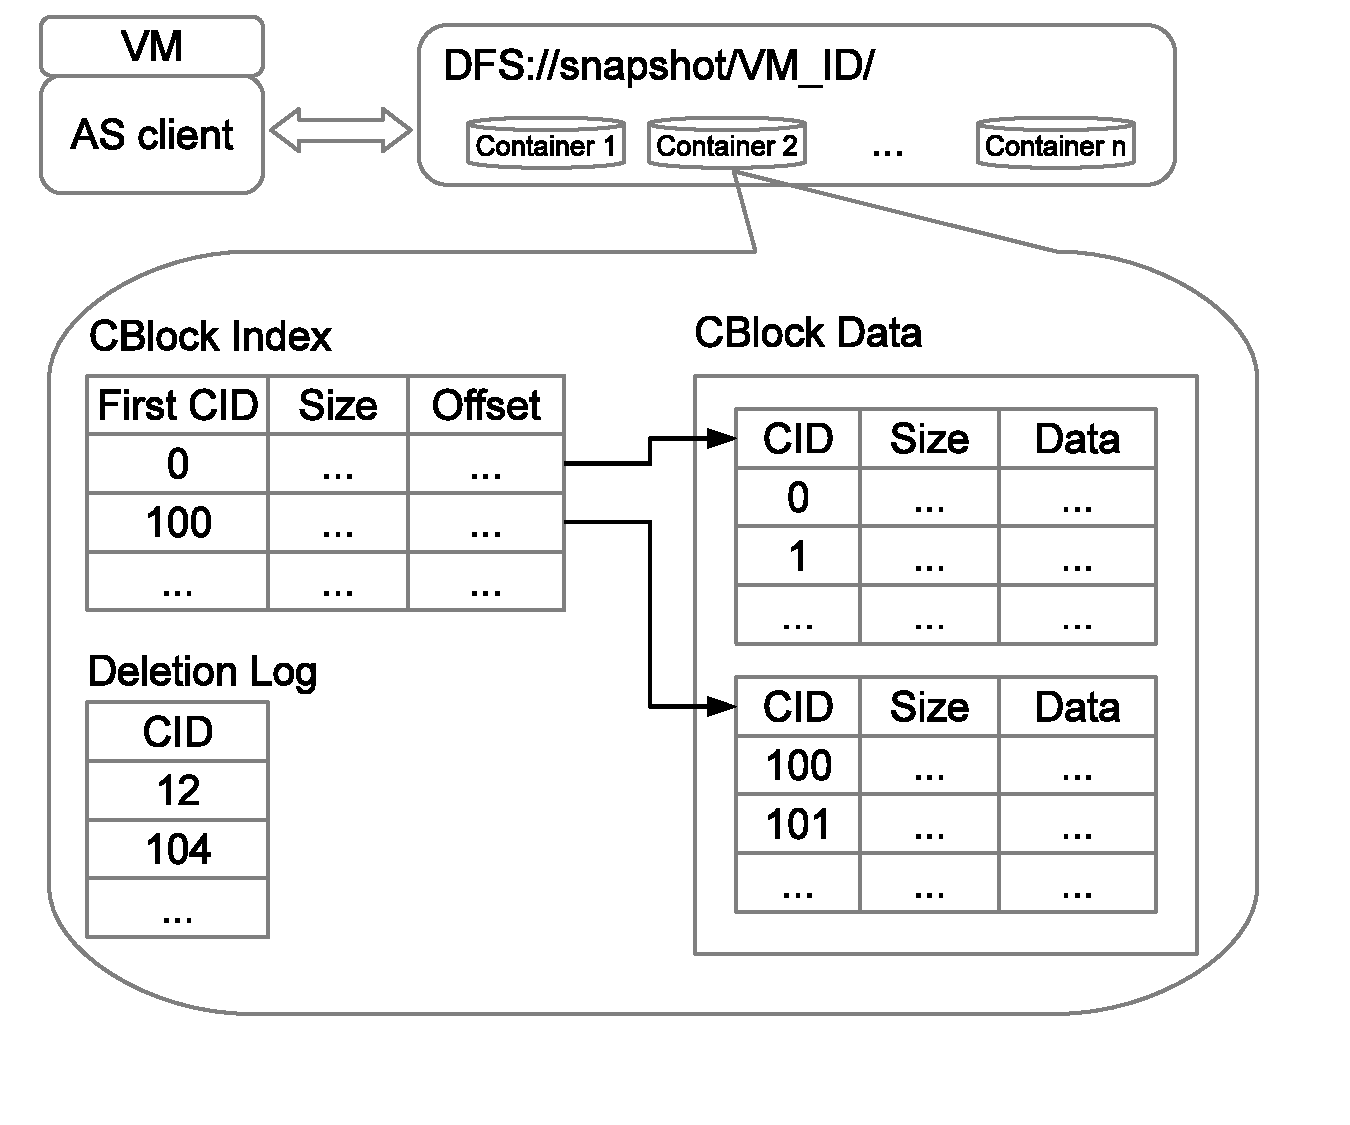
\epsfig{file=images/append_store_arch.pdf, width=3.5in}
  \caption{Architecture of Append Store}
  \label{fig:as_arch}
\end{figure}

Append Store supplies three interfaces: {\em get(ref)} accepts a data reference and retrives data, 
{\em put(data)} accepts data and returns a reference to be stored in metadata recipes, 
{\em delete(ref)} 
deletes the data pointed by the reference.
Under the hood, small var-sized data are grouped and stored into larger data containers. Each VM has
its snapshot data stored in its own Append Store, specified by the VM ID. 
We split every Append Store into multiple data containers so that reclaiming the disk space would not 
result in rewriting all the data at the same time.

As shown in Fig.\ref{fig:as_arch}, every data container is represented as three data files in DFS:
the data file holds all the actual data, the index file is responsible for translating data reference
into data locations, and a deletion log file remembers all the deletion requests to the container.

A data reference is composed of two parts: a container ID (2 bytes) and CID (6 bytes).
Append Store assign every piece of data a CID for its internal data referencing. 
When new data is appended, its CID is the current largest CID in that container plus one.
As a result, all the data locations are naturally indexed by this self-incremental CID, 
no extra sorting is needed.

Append Store groups multiple chunk data (i.e., 100) into larger units, called {\em CBlock}.
CBlock is the basic unit for append store's internal read/write/compression.
There is one index entry in the container index corresponding to every CBlock. It keeps the first chunk's CID
in that CBlock, and the CBlock data's size and location.

Using CBlock brings us several advantages: First, the write workload to DFS master is greatly reduced; second, grouping
small chunks gives better compression. Third, reading a CBlock (200 - 600 KB) typically cost the same amount of disk 
seek as reading a 4KB chunk. Finally, this greatly reduces the size of index. Let $m$ be the number of chunks in each
CBlock, then the overall index size is reduced to $1/m$. In our implementation, using $m=100$ reduces the index for
a 1GB container from 10 MB to 100 KB.

\subsection{Operations}
In order to read a chunk data by reference, Append Store client first loads the
container index file specified by the container ID, then search the CBlock index to find the entry that covers the chunk by CID.
After that, it reads the whole CBlock data from DFS, decompress it, seek the exact chunk data specified by CID. 
Finally, the client updates itws internal chunk data cache with the newly loaded contents to anticipate future sequential reads.

Write requests to append store are accumlated. When the number reaches $m$, the AS client forms a CBlock by assigning 
every chunk a CID, compress the CBlock data, and append it to the CBlock data file. Then a new CBlock index entry is appended
to CBlock index.

Append store adopts lazy delete strategy. The deletion requests are appended into every container's deletion log file with the CID of data to be deleted.
CIDs in deletion log are guaranteed to be referenced by nobody and can be safe deleted in future. 
Periodically, snapshot management system asks append store to compact containers in order to reclaim disk space. 
The actual compaction will only take place when the number of deleted items reached $d\%$ of container's capacity. 
During compaction, append store creates a new container (with the same container ID) to replace the 
existing one. This is done by sequentially scan the old container, copying all the chunks that are not 
found in deletion log to the new container, creating new CBlocks and indices. 
However, every chunk's CID is plainly copied rather than re-generated. This does not affect the sorted
order of CIDs in new container, but just leaving holes in CID values. As the result, all data references stored 
in upper level recipes are unaffected, and the data reading process is as efficient as before.

%hard problems

\subsection{Analysis}

Snapshot operation performance analysis:
\begin{table}
    \begin{tabular}{l p{1.5in} l}
        \hline
        Symbol & Description & Measurement \\ \hline
        $N_{seg}$ & Number of segments in the snapshot & ~ \\ [1ex] \\ [-1.5ex]
        $N_{chunk}$ & Number of chunks in one segment & ~ \\ [1ex] \\ [-1.5ex]
        $P_{dirty}$ & Probablity of a segment is dirty & ~ \\ [1ex] \\ [-1.5ex]
        $P_{new}$ & Percentage of new data & ~ \\ [1ex] \\ [-1.5ex]
        $P_{change}$ & Probablity that a chunk is not found in parent snapshot & ~ \\ [1ex] \\ [-1.5ex]
        $P_{in\_CDS}$ & Percentage of chunks in CDS & ~ \\ [1ex] \\ [-1.5ex]
        $T_{scan}$ & Time to scan segment data and caculate content hash & 74 ms \\ [1ex] \\ [-1.5ex]
        $T_{write\_AS}$ & Time of writing a chunk into append store & 0.24 ms \\ [1ex] \\ [-1.5ex]
        $T_{read\_AS}$ & Time of reading a chunk from append store & ~ \\ [1ex] \\ [-1.5ex]
        $T_{read\_chunk}$ & Time of reading a chunk & ~ \\ [1ex] \\ [-1.5ex]
        $T_{check\_CDS}$ & Time of checking CDS & ~ \\ [1ex] \\ [-1.5ex]
        $T_{read\_CDS}$ & Time of reading a chunk data from CDS data store& ~ \\
        \hline
    \end{tabular}
    \caption{List of performance factors}
    \label{tab:as_param}
\end{table}

The overall time of writing a snapshot is:

\begin{dmath}
T_{write} = P_{dirty} * N_{seg} * [max(T_{scan}, T_{read\_AS}) + P_{change} * N_{chunk} * T_{check\_CDS} + P_{new} * N_{chunk} * T_{write\_AS}]
\end{dmath}

The overall time to read a snapshot is:

\begin{dmath}
T_{read} = N_{seg} * {T_{read\_AS} + N_{chunks} * [P_{in\_CDS} * T_{read_CDS} + (1 - P_{in\_CDS}) * T_{read\_chunk}]}
\end{dmath}

Average time of reading a chunk:

\begin{dmath}
T_{read\_chunk} = P_{in\_CDS} * T_{read\_CDS} + (1 - P_{in\_CDS}) * T_{read\_AS}
\end{dmath}

Time of reading append store:

\begin{dmath}
T_{read\_AS} = 0 * P_{in\_cache} + (1 - P_{in\_cache} ) * T_{load\_CBlock}
\end{dmath}
